% This is samplepaper.tex, a sample chapter demonstrating the
% LLNCS macro package for Springer Computer Science proceedings;
% Version 2.20 of 2017/10/04
%
\documentclass[runningheads]{llncs}
%
\usepackage{graphicx}
\usepackage{todonotes}
\usepackage{verbatim}
\usepackage{caption}
\usepackage{hyperref}
% Used for displaying a sample figure. If possible, figure files should
% be included in EPS format.
%
% If you use the hyperref package, please uncomment the following line
% to display URLs in blue roman font according to Springer's eBook style:
% \renewcommand\UrlFont{\color{blue}\rmfamily}

\begin{document}
%
\title{Clustering Knowledge Graphs}
%
%\titlerunning{Abbreviated paper title}
% If the paper title is too long for the running head, you can set
% an abbreviated paper title here
%
\author{Lina Teresa Molinas Comet}
%
\authorrunning{Lina Teresa Molinas Comet.}
% First names are abbreviated in the running head.
% If there are more than two authors, 'et al.' is used.
%
\institute{RWTH Aachen University, Aachen, Germany \\
\email{lina.molinas.comet@rwth-aachen.de}\\
\url{http://dbis.rwth-aachen.de/cms}}
%
\maketitle              % typeset the header of the contribution
%
\begin{abstract}
We are living in the big data era, dealing with big amounts of data available in different format representations. Among those representations, stands out one of the most valuable approaches for data representation, the use of graph like structures, which allows information integration from multiple sources. Moreover, clustering techniques are use on top of graphs to group information based on their similarity or other relevant characteristics. As a consequence, it is essential to analyze different clustering methods to implement in a particular scenario to get the most from knowledge-base representations. For this reason, in this paper we present an overview of the most interesting new techniques and algorithms for clustering knowledge graphs. We also provide an analysis comparing and contrasting those approaches.

\keywords{Knowledge Graphs \and Clustering \and Knowledge Bases \and Algorithms}
\end{abstract}
%
%
%
\section{Introduction} \label{introduction}
We are living in the big data era, meaning that we need to deal with big amounts of data available in different format representations. In order to get valuable insights it is not enough accessing it, but extracting the right portion of data to help us make sense of the beneath information \cite{Pedrycz}. However, the extracting process is not an easy task due to the resulting complexity of having different data representations, and the underlying semantics that may be lost in the process. One way of dealing with this kind of problems is using graph-based data representation which allows information integration from multiple structured or unstructured sources sources.
Although data representation is important, is not the only requisite for dealing with data. It is equally important to apply the right procedures to get valuable insights by exploring large datasets. One of those techniques is clustering data in order to group similar entities.  In this sense, it is essential to analyze and compare different clustering techniques and algorithms to implement in a particular scenario to get the most from knowledge-base representations \cite{Pedrycz}.

For these reasons, our contribution in this paper is presenting an overview of the most interesting new techniques and algorithms for clustering knowledge graphs. Furthermore we also provide an analysis comparing and contrasting those different approaches.

The structure of this paper is as follows: first, in section \ref{background} we introduce some concepts related to the topic. Then, in section \ref{general-techniques}, we briefly look at some traditional clustering approaches and the common problems on graph clustering (e.g. overlapping). After that, in section \ref{algorithms}, we revise in more details some of the new techniques and algorithms developed for graph clustering in the web.

Finally, in sections \ref{analysis} and \ref{discussion} we critically discuss the different techniques by comparing them, as well as providing suggestion of application areas for the betterment of data grouping. 


\section{Background} \label{background}
First of all, for a better understanding, in this section we define the main concepts related to the topic under study. After that, we provide a short description of the relation between those concepts.


\subsection{Graphs} \label{graphs}
In the formal definition of Diestel \cite{Diestel}, ``a $graph$ is a pair $G = (V, E)$ of sets satisfying $E \subseteq [V]^2$; thus, the elements of $E$ are 2-element subsets of $V$". He also indicates that ``the elements of $V$ are the $vertices$ (or $nodes$ or $points$) of the graph $G$, the elements of $E$ are its $edges$ (or $lines$)".

In other words, a graph is a set of vertices (nodes) and edges (links) connecting those vertices. The nodes on a graph represent different entities from the real world \cite{Robinson}, while the edges depict the relationship among them.

\subsection{Knowledge Graphs} \label{knowledge-graphs}
Currently there is not a common definition of the term knowledge graphs (KG). Neither exist, as explained for Ehrlinger and W{\"o}{\ss} \cite{Ehrlinger}, an exact differentiation between the use of this term and the others related (i.e. knowledge bases, knowledge vault, and ontology). What is more, Google has its own implementation of what they call Knowledge Graph\footnote{Introducing the Knowledge Graph: things, not strings, accessed December 12, 2018,  \href{https://googleblog.blogspot.com/2012/05/introducing-knowledge-graph-things-not.html}{https://googleblog.blogspot.com/2012/05/introducing-knowledge-graph-things-not.html}}, which is an ``intelligent model" that understands some semantics and helps the search engine to create a short summary related to a topic, but which does not cover all the aspects considered in a KG according to other interpretations of the term \cite{Ehrlinger}.

In the definition of Paulheim \cite{Paulheim}, ``a knowledge graph
1. mainly describes real world entities and their interrelations, organized in a graph, 2. defines possible classes and relations of entities in a schema, 3. allows for potentially interrelating arbitrary entities with each other, and 4. covers various topical domains". A more formal definition, which also focuses more on the context of the Semantic Web, is proposed by F{\"a}rber \cite{Farber}: ``we define a Knowledge Graph as an RDF Graph. An RDF graph consists of a finite set of RDF triples where each RDF triple $(s, p, o)$ is an ordered set of the following RDF terms: a subject $s \in U ∪ B$, a predicate $p \in U$, and an object $o \in U ∪ B ∪ L$. An RDF term is either a URI $u \in U$, a blank node $b \in B$, or a literal $l \in L$. $U, B,$ and $L$ are infinite sets and pairwise disjoint".

Additionally, Ehrlinger and W{\"o}{\ss} \cite{Ehrlinger} propose the following definition: ``a knowledge graph acquires and integrates information into an ontology and applies a reasoner to derive new knowledge.". Moreover, they suggest that knowledge graphs involve the use of a graph-based structure to store data. However, KG focus on the instances rather than on the schema of the represented knowledge \cite{Paulheim}


\subsection{Knowledge-based systems} \label{knowledge-based}
A knowledge-based system is also called an expert system, and is part of one of the areas of Artificial Intelligence (AI) \cite{Tripathi}. More specifically, Engelmore \cite{Engelmore} suggests that a knowledge base is a database containing facts, rules, and relations. Additionally, Tripathi \cite{Tripathi} points out that expert systems aim to acquire expert knowledge coming from a human who is an specialist in a particular domain, and subsequently making that information available to non-expert users.
Therefore, using an expert system can lead to benefits in handling knowledge, and as Engelmore \cite{Engelmore} mentions, one of its key profits is the quality improvement of tasks related to decision making.


\subsection{Clustering} \label{clustering}
Clustering is a field of study which helps to discover and expose known or unknown clusters in datasets \cite{Han} \cite{Mirkin}.

Clustering aims to divide an object (dataset) into various groups (clusters) relying on the entities' attributes. After the division, the entities in one group are highly similar, while are quite different to the entities in other groups \cite{Han}.

Clustering is useful for coping with big amount of data by helping data analysis \cite{Pedrycz} \cite{Mirkin}. Therefore, it is used in many application areas, such as engineering, economics, biology, business intelligence, web search, pattern recognition, etc. \cite{Pedrycz} \cite{Han}; and can be seen from many different perspectives (e.g. machine learning, data mining, knowledge-discovery, statistics,etc.). In this respect, those perspectives can also overlap as we will see in this paper, in the section \ref{algorithms}.


\subsection{Interrelation of terms} \label{interrelation}
We previously mentioned Engelmore's remarks about the benefits of using knowledge-based systems. Likewise, implementing knowledge graphs is rewarding, as shown by the use in industry. In this context, Pan et al. \cite{Pan} introduce some success cases involving KG to first collect and then provide not only data but knowledge. As a result, KG help knowledge-based search services to discover and understand information.
Moreover, from the Linked Data perspective, this involve linking content with meaning for a better topic understanding \cite{Pan}.

As Tang et al. \cite{Tang} present, clustering can be use to group knowledge based on content similarity. Hence, to find related topics for a specific application (e.g. common topics between two people interchanging emails).

In summary, clustering techniques support knowledge graphs by associating related content, and with this improving data exploration and knowledge discovery.


\section{State of the Art}\label{state-art}
In this section we present novel and also more traditional techniques and algorithms used in the field of Knowledge Graph clustering. 

The system divides a set of instances into clusters or groups based on some measure of similarity. There are two main types of clustering algorithms. And there are 2 types of clustering algorithms: k-means clustering, and hierarchical clustering, where the first one is ... and for the second approach it is not necessary to specify the desired number of clusters but instead the clustering are built in each iteration grouping  the similar clusters (first those where individual clusters)\cite{Zacharski}

\todo{look at different types of clustering: agglomerative https://www.linkedin.com/pulse/types-cluster-analysis-techniques-k-means-using-r-irrfan-khan/}

\subsection{General Techniques for Knowledge Graph Clustering} \label{general-techniques}
Presentation of well-known techniques for graph clustering.


\subsection{Techniques and Algorithms}\label{algorithms}
Revision in more detail the selected algorithms and techniques 


\subsubsection{Graph clustering for content aggregation for an Ontology-Based P2PKM}\label{content-aggregation}
Present the work of \cite{Schmitz} where they introduce the approach of semantic self-descriptions to be publish among peers and for which they use a clustering algorithm to obtain that self-description.


\subsubsection{Structural similarity clustering entities} \label{structural-similarity}


\subsubsection{Entity Clustering using link features} \label{entity-clustering}


\begin{center}
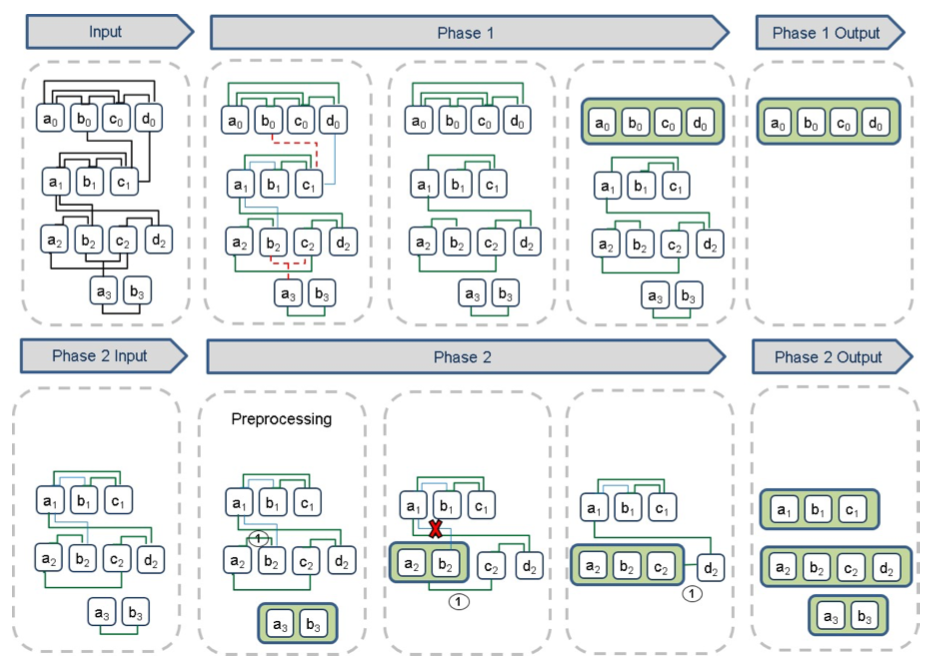
\includegraphics[width=1\textwidth]{clip_example.png}
\captionof{figure}{Example of CLIP \cite{Saeedi}}
\end{center}

\begin{center}
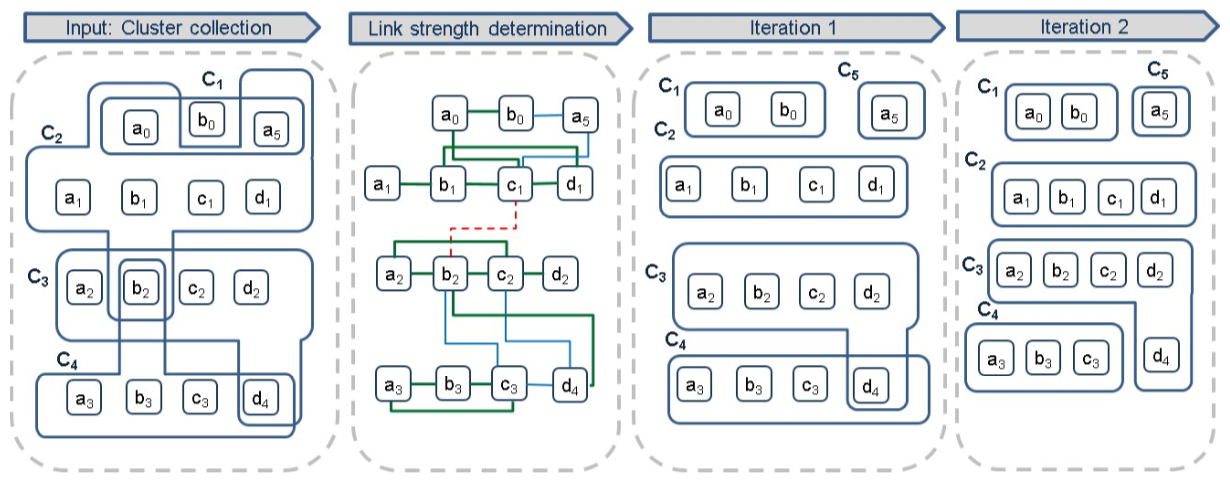
\includegraphics[width=1\textwidth]{clip_overlap_resolution.png}
\captionof{figure}{Overlapping resolution on CLIP \cite{Saeedi}}
\end{center}


\section{Analysis and comparison of presented approaches} \label{analysis}
\section{Discussion} \label{discussion}
\section{Conclusion} \label{conclusion}

%
% ---- Bibliography ----
%
% BibTeX users should specify bibliography style 'splncs04'.
% References will then be sorted and formatted in the correct style.
%
\bibliographystyle{splncs04}
\bibliography{mybibliography}
%
\begin{thebibliography}{8}
\bibitem{Schmitz}
Schmitz, C., Hotho, A., J{\"a}schke, R., Stumme, G.: Content Aggregation on Knowledge Bases Using Graph Clustering. In: Sure, Y., Domingue, J. (eds.) The Semantic Web: Research and Applications. ESWC 2006, LNCS, vol. 4011, pp. 530--544.
Springer, Berlin, Heidelberg (2006). \doi{10.1007/11762256\_39}

\bibitem{Elbattah}
Elbattah, M., Roushdy, M., Aref, M., M.Salem, A.: Large-Scale Entity Clustering Based on Structural Similarity within Knowledge Graphs. In: Arun, K., Somani, G. (eds.) Big Data Analytics: Tools and Technology for Effective Planning, Edition: 1, Chapter: 14, pp. 311--334. CRC Press Editors (2017). \doi{10.1201/b21822-14}

\bibitem{Saeedi}
Saaedi, A., Peukert, E., Rahm, E.  : Using Link Features for Entity Clustering in Knowledge Graphs. In: Gangemi, A., Navigli, R., Vidal, M., Hitzler, P., Troncy, R., Hollink, L., Tordai, A., Alam, M. (eds.) The Semantic Web. ESWC 2018, LNCS, vol. 10843, pp. 576--592.
Springer International Publishing, Cham (2018). \doi{10.1007/978-3-319-93417-4\_37}

\bibitem{Pedrycz}
Pedrycz, W.: Knowledge-Based Clustering: From Data to Information Granules. 2nd edn. Wiley-Interscience, New York, NY, USA (2005)

\bibitem{Zhang}
Zhang, X., Lv, Y., Lin, E : Object Clustering in Linked Data using Centrality. In: Proceedings of China Conference on Knowledge Graph and Semantic Computing (CCKS2016)
on Proceedings, pp. 172--183. Publisher, Location (2016). \doi{10.1007/978-981-10-3168-7\_17}

\bibitem{Ehrlinger}
Ehrlinger, L, W{\"o}{\ss}, W.: Towards a Definition of Knowledge Graphs. In: Martin, M., Cuquet M., Folmer, E. (eds.) In Joint Proceedings of the Posters and Demos Track of the 12th International Conference on Semantic Systems - SEMANTiCS2016 and the 1st International Workshop on Semantic Change \& Evolving Semantics (SuCCESS'16), CEUR-WS, vol. 1695, Leipzig, Germany (2016). \doi{10.10007/1234567890}

\bibitem{Paulheim}
Paulheim, H.: Knowledge Graph Refinement: A Survey of Approaches and Evaluation Methods. Semantic Web Journal, 489--508 (2017). \doi{10.3233/SW-160218}

\bibitem{Farber}
F{\"a}rber, M., Bartscherer, F, Menne,C., Rettinger, A.: Linked data quality of DBpedia, Freebase, OpenCyc, Wikidata, and YAGO. Semantic Web Journal, 77--129 (2018). \doi{10.3233/SW-170275}

\bibitem{Tripathi}
Tripathi, K.: A Review on Knowledge-based Expert System: Concept and Architecture. IJCA Special Issue on Artificial Intelligence Techniques-Novel Approaches \& Practical Applications (2011). \doi{10.5120/2845-226}

\bibitem{Engelmore}
Engelmore R.S.  : Artificial Intelligence and Knowledge Based Systems: Origins, Methods and Opportunities for NDE. In: Thompson D.O., Chimenti D.E. (eds.) Review of Progress in Quantitative Nondestructive Evaluation. Review of Progress in Quantitative Nondestructive Evaluation, vol. 6 A., 
Springer, Boston, MA (1987). \doi{10.1007/978-1-4613-1893-4\_1}

\bibitem{Diestel}
Diestel, R.: Graph Theory. 4th edn. Springer, New York, NY, USA, (2012)

\bibitem{Robinson}
Robinson, I., Webber, J.,Eifrem, E.: Graph Databases. 2nd edn. O'Reilly Media, Inc., Sebastopol, CA (2015)

\bibitem{Pan}
Pan, J., Vetere, G., Gomez-Perez, J., Wu,: Exploiting Linked Data and Knowledge Graphs in Large Organisations. 1st edn. Springer International, Switzerland, (2017)

\bibitem{Zacharski}
Zacharski, R.: A Programmer's Guide to Data Mining. http://guidetodatamining.com/, (2012)

\bibitem{Han}
Han, J., Kamber, M., Pei, J.: Data Mining: Concepts and Techniques. 3rd edn. Morgan Kaufmann Publishers Inc.,
San Francisco, CA, USA (2011)

\bibitem{Mirkin}
Mirkin, B.: Clustering For Data Mining: A Data Recovery Approach. 2nd edn. Chapman \& Hall/CRC,
Boca Raton, FL, USA (2005)

\bibitem{Tang}
Tang, G., Pei, J., Luk, W.: Email Mining: Tasks, Common Techniques, and Tools. Knowl. Inf. Syst., 1--31 (2014). \doi{10.1007/s10115-013-0658-2}

\end{thebibliography}

\begin{comment}
\bibitem{ref_lncs1}
Author, F., Author, S.: Title of a proceedings paper. In: Editor,
F., Editor, S. (eds.) CONFERENCE 2016, LNCS, vol. 9999, pp. 1--13.
Springer, Heidelberg (2016). \doi{10.10007/1234567890}

\bibitem{ref_article1}
Author, F.: Article title. Journal \textbf{2}(5), 99--110 (2016)

\bibitem{ref_book1}
Author, F., Author, S., Author, T.: Book title. 2nd edn. Publisher,
Location (1999)

\bibitem{ref_proc1}
Author, A.-B.: Contribution title. In: 9th International Proceedings
on Proceedings, pp. 1--2. Publisher, Location (2010)

\bibitem{ref_url1}
LNCS Homepage, \url{http://www.springer.com/lncs}. Last accessed 4
Oct 2017

\end{comment}
\end{document}


